
\chapter{基于粒子群算法的软件补偿方法及算法硬化}
\section{粒子群算法}
\subsection{粒子群算法基本原理}

粒子群算法(Particle Swarm optimization,PSO)是一种启发于鸟群协同捕食行为的智能算法,利用种群与个体之间的信息交互来寻找问题的最优解,具有较高的搜索效率和精度\cite{潘红丽2022基于改进粒子群算法的垃圾清运车辆低碳路径规划},已广泛应用于函数优化等领域\cite{2022Environmental}。
\begin{figure}[htb]
  \centering
  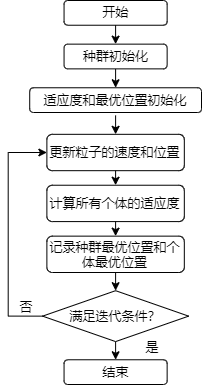
\includegraphics[width=4cm,height=7cm]{fig/4-fig/粒子群算法流程图.png}
  \caption{粒子群算法流程图}
  \label{fig:粒子群算法流程图}
\end{figure}
可以假设这样一个场景:一群鸟在随机的搜寻食物,并且搜寻空间里只有一块食物,所有的鸟都不知道食物在哪里,并且所有鸟的初始位置和搜寻方向都是随机的。在该场景下,一个找寻食物的最优策略就是搜寻离食物最近的鸟的周围。距离食物的距离就代表着优化效果的好坏,而鸟群每个时刻所处在的位置,就代表着粒子群算法覆盖到的迭代值,整个空间即为粒子群算法的搜索空间,将该方式抽象成算法,如图\ref{fig:粒子群算法流程图}所示。

由图\ref{fig:粒子群算法流程图}中可以看出,粒子群算法的第一步是对种群进行初始化,即设定优化对象的迭代起点,并根据目标函数计算出与起点对应的适应度(Fitness,下文简称fit),并在所有个体的适应度中筛选出最优的,用其对应的迭代起点作为整个种群目前的种群最优解(Global best,下文简称gbest),而所有个体的个体最优解(Person best,下文简称pbest),这样就完成了整个算法的初始化。随后使用gbest、pbest对粒子的速度和位置更新进行控制,使迭代方向不断朝着最优的方向进行,即上述“搜寻离食物最近的鸟的周围”的策略,具体的速度更新公式和位置更新公式如下式所示:
\begin{equation}\label{eq:粒子群算法速度更新}
  V^{k+1}_i=\omega V^{k}_i\,+\,c_pr_{and}(pbest_i-X^{(k)}_i)+c_gr_{and}(gbest\,-\,X^{(k)}_i).
\end{equation}
\begin{equation}\label{eq:粒子群算法位置新}
    X^{k+1}_i\,=\,X^{(k)}_i\,+\,V_i^{k+1}.
\end{equation}

上式中\(V^{k}_i\)和\( X^{k}_i\)中分别表示粒子的速度和位置,下标i表示种群中第i个粒子,上标(k+1)表示当前种群为第(k+1)次迭代,\(\omega\)称为惯性因子,是一个衡量全局寻优能力和局部寻优能力的非负参数;\(c_p\)和\(c_g\)为非负常数,通常设为2;、\(r_{and}\)为[0,1]范围内的随机数,\(pbest_i\)为第个粒子的个体历史最优位置,gbest为整个种群的历史最优位置。

\subsection{线性惯性权值递减策略}
由式\eqref{eq:粒子群算法速度更新}可以看出惯性因子主要控制粒子的历史速度对当前速度的影响,历史速度在当前速度中占比大,则速度的更新将主要集中在历史速度附近,此时粒子群算法的局部寻优能力较强,并且收敛速度较快;若历史速度在当前速度中占比小,则速度的更新将在整个搜索域中进行,此时粒子群算法的全局寻优能力较强,使得搜索结果容易跳出局部优值。

为了在迭代初期,能够有更好的全局寻优能力,尽可能找到搜索域中所有可能的最优解,在迭代后期拥有更好的局部寻优能力,以便快速收敛,在惯性因子的取值上采用线性递减策略\cite{冯浩2015一种改进的粒子群优化算法惯性权值递减策略},即惯性因子\(\omega\)由下式更新。
\begin{equation}\label{eq:omega更新公式}
  \omega^k\,=\,\omega_e\,+\,\frac{(\omega_i\,-\,\omega_e)(k_{max}\,-\,k)}{k_{max}}.
  \end{equation}

其中\(\omega_i\)和\(\omega_e\)分别为迭代开始时的惯性因子和迭代结束时的惯性因子,\(k_{max}\)为最大迭代次数,k为当前的迭代次数。通过对惯性因子使用线性递减策略,可以在迭代过程中不断调整全局寻优能力和局部寻优能力。

但是粒子群算法存在早熟收敛的问题,即当粒子群到达局部最优解附近时,粒子速度的更新主要由自身速度决定,并且由于粒子群算法的惯性因子\(\omega^k\)通常小于1,使得粒子速度的更新幅度将会越来越小,难以跳出该局部最优解\cite{范培蕾2009克服早熟收敛现象的粒子群优化算法}。

虽然Edlen公式的诞生方法使其补偿精度和使用条件受到一定影响,但原始的Edlen公式为PSO算法提供了一个优秀的搜索起点,相当于大幅压缩了PSO算法的搜索空间,这能非常有效地避免早熟收敛问题的出现。

\section{基于粒子群算法优化后的Edlen公式补偿方法}
为了解决上述的Edlen公式存在的问题,本文提出一种使用粒子群算法对Edlen公式进行优化的方法。

对于粒子群算法而言,目标函数的形式会严重影响算法优化的结果,而Edlen公式作为一个几十年来广泛使用的经验公式,虽然由于其诞生条件的局限性使得其使用范围受限,但Edlen公式的形式仍然具有重要的借鉴意义,将Edlen公式与粒子群算法相结合,不仅可以有效地避免粒子群算法寻找到局部最优解,避免早熟收敛现象的发生,还可以减小搜索空间,减小收敛时间,保证训练时不会影响实时数据测量及补偿。
\subsection{数据预处理}
使用粒子群算法对Edlen公式进行优化的第一步是对位移、温度、气压数据进行预处理,这点主要是基于下面两点考虑:
\begin{enumerate}
  \item 虽然所有被测量的采样周期均为$2s$,但是由于位移测量的上位机采用C-SHOP编写,而温度测量的上位机是基于LabVIEW开发的,气压测量主要依靠PACE1000气压传感器,这导致三者在定时功能上可能会有细微差别,而导致最终采样的点数不相同,所需要进行数据的裁剪。
  \item 出于不漏采任何有效信息,所以将采样周期设置为$2s$,但是温度和气压都是缓变量,并不可能在这么短的时间内明显变化,所以为了数据的可靠性,避免偶然性数据造成训练效果降低,需要对数据进行均值滤波。
\end{enumerate}
在进行数裁剪的时候采用如下策略:将位移、温度、气压三组中数据个数最少的作为基准,计算另外两组数据个数与基准的差值,这个差值即为需要裁剪的数据个数,将数据个数除以裁剪个数,然后向下取整即可得到每组数据对应的裁剪窗口长度,在每个裁剪窗口内将最后两个数取平均值,用平均值代替这两个数,这样即可实现数据裁剪。

在进行均值滤波的时候采用如下策略:取窗口长度为$30s$,即15个数据点,在整个数据段内进行滑动窗口的均值滤波。

\subsection{使用粒子群算法进行数据训练}
将式\eqref{eq:线性形式的Edlen公式}作为粒子群算法的目标函数,温度因子$\frac{\delta n}{\delta T}$和气压因子$\frac{\delta n}{\delta P}$作为两个搜索目标,第一次迭代的搜索起点分别为$-9.36*10^{-7}$和$2.68*10^{-9}$,即搜索点由下式更新:
\begin{equation}\label{eq:搜索点更新公式}
  \delta^{(n+1)}_i = \delta^{(n)}_i+(\delta^{(n)}_o-\delta^{(n)}_i).
  \end{equation}

式\eqref{eq:搜索点更新公式}中$\delta^{(n+1)}_i$为第$n+1$次训练时温度因子、气压因子初始搜索点,即$\delta_i\,=\,(\frac{\delta n}{\delta T}\,\,\,\frac{\delta n}{\delta P})$,所以该式描述的是第$n+1$的搜索起点与第$n$次搜索起点之间的关系。特别地,当$n=0$时,即第一次搜索的搜索起点为$\delta_i\,=\,(-9.36*10^{-7}\,\,\,2.68*10^{-9})$,即原始Edlen公式的温度因子值和气压因子值。$\delta_o^{(n)}$为第$n$次训练后粒子群算法计算出的温度因子和气压因子。

而每次训练计算$\delta_o^{(n)}$的适应度时,采用均方根误差作为评价指标,其计算方法如式\eqref{eq:均方根误差计算公式}所示:
\begin{equation}\label{eq:均方根误差计算公式}
  RMSE = \sqrt{\frac{\sum_{i=1}^{N}(x-\widehat x)^2}{N}}.
  \end{equation}

\section{整段式粒子群算法补偿效果}
将一整组的测量数据作为粒子群算法的训练样本,从给定的搜索起点开始,根据式\eqref{eq:均方根误差计算公式}计算初始适应度,并且进行种群最优位置和个体最优位置的初始化,然后根据式\eqref{eq:粒子群算法速度更新}和式\eqref{eq:粒子群算法位置新}更新种群中所有个体的速度和位置,然后循环迭代多次,直至适应度满足要求或者达到迭代上限,此时种群的最优位置即为粒子群算法优化后的Edlen公式中的温度因子和气压因子,然后对测量数据进行补偿。训练样本统一使用测量臂长度$90nm$的干涉仪的测量数据,使用优化结果对测量臂长度$45nm$和$90nm$测量数据同时进行补偿,补偿结果如下。

\subsection{短时测量}
如图\ref{fig:粒子群算法优化后的短时测量补偿效果}所示,(a)图为测量臂长度为$45nm$的位移测量数据,(b)图为测量臂长度为$90nm$的位移测量数据,(c)图为对应的温度和气压数据,(a)、(b)、(c)三图的横轴均为时间,单位为h;(a)和(b)图中的竖轴为位移数据,单位为$nm$,其中带圆圈标注的蓝色曲线为原始的位移测量数据,带黄色方块标注的为使用原始Edlen公式补偿后的位移数据,带红色菱形标注的为使用粒子群算法优化后的补偿后位移数据,(c)图的竖轴为温度和气压数据,单位为$^{\circ}C$和$kPa$,其中带圆圈标注的蓝色曲线为温度数据,红色曲线为气压数据。
\begin{figure}[htb]
    \centering
    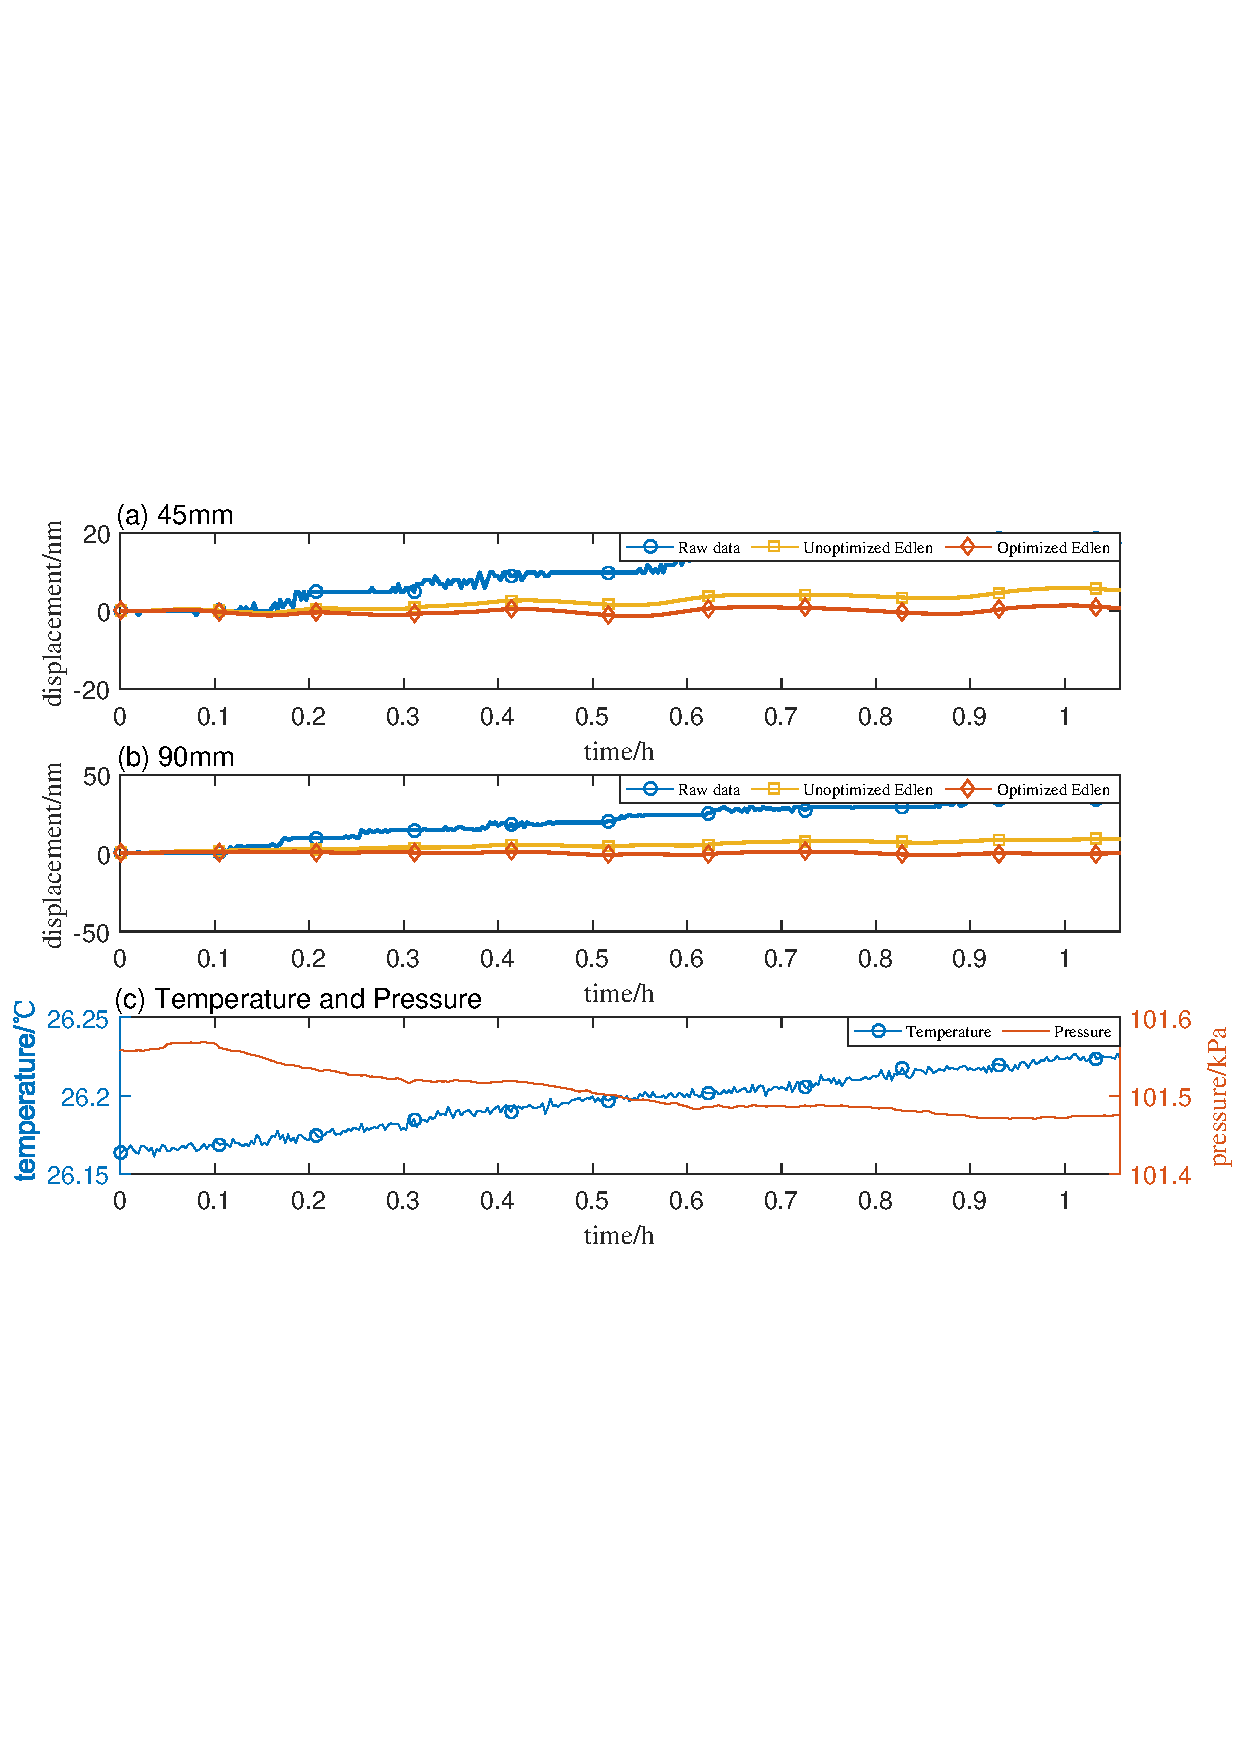
\includegraphics[width=14cm]{fig/4-fig/edpso_短时测量实验数据.pdf}
    \caption{粒子群算法优化后的短时测量补偿效果}
    \label{fig:粒子群算法优化后的短时测量补偿效果}
\end{figure}

如图\ref{fig:粒子群算法优化后的短时测量补偿效果}所示,优化后的红色曲线相比于未经优化的黄色曲线,无论是$45nm$还是$90nm$情况下,都更加接近于理论位移值$0nm$,这说明使用粒子群算法对Edlen公式进行优化之后在进行补偿可以比较明显地提升补偿效果。从数据层面分析,使用粒子群算法进行优化之后再进行补偿,测量臂长度为$45nm$的干涉仪的残留均方根误差从$3.1377nm$降低为$0.8541nm$,而$90nm$长度的则从$5.8401nm$降低为$1.034nm$,分别同比减小了$72.7\%$和$82.3\%$,并且两者残差的差值只有$0.1799nm$,相较于未优化前的差值$2.7024nm$有着较大提升,可以认为使用经过粒子群算法优化之后的Edlen公式进行补偿后的残差在不同测量臂长度情况下是近似相等的,这说明环境误差得到了比较精准并且完全的补偿。但是如果从百分比的角度分析,$0.1799nm$的残差差值占原始残差的比例约为$21\%$,这是一个比较大的百分比,可能的原因是由于改组温度变化较小,使得环境误差在总体误差中的比例不够大。

\subsection{长时测量}
对前文所述的长时测量的实验数据也是用粒子群算法优化后再进行补偿,结果如图\ref{fig:粒子群算法优化后的长时测量补偿效果}所示,虽然采样时长增加了,但是粒子群算法的优化效果依旧显著。从数据层面分析,使用粒子群算法进行优化之后再进行补偿,测量臂长度为$45nm$的干涉仪的残留均方根误差从$14.9957nm$降低为$6.8308 nm$,而$90nm$长度的则从$43.5806nm$降低为$3.6700nm$,两者残差的差值只有$3.16nm$,相较于未优化前的差值$28.5849nm$有着较大提升,可以认为使用经过粒子群算法优化之后的Edlen公式进行补偿后的残差在不同测量臂长度情况下是近似相等的,这说明环境误差得到了比较精准并且完全的补偿。
\begin{figure}[htb]
  \centering
  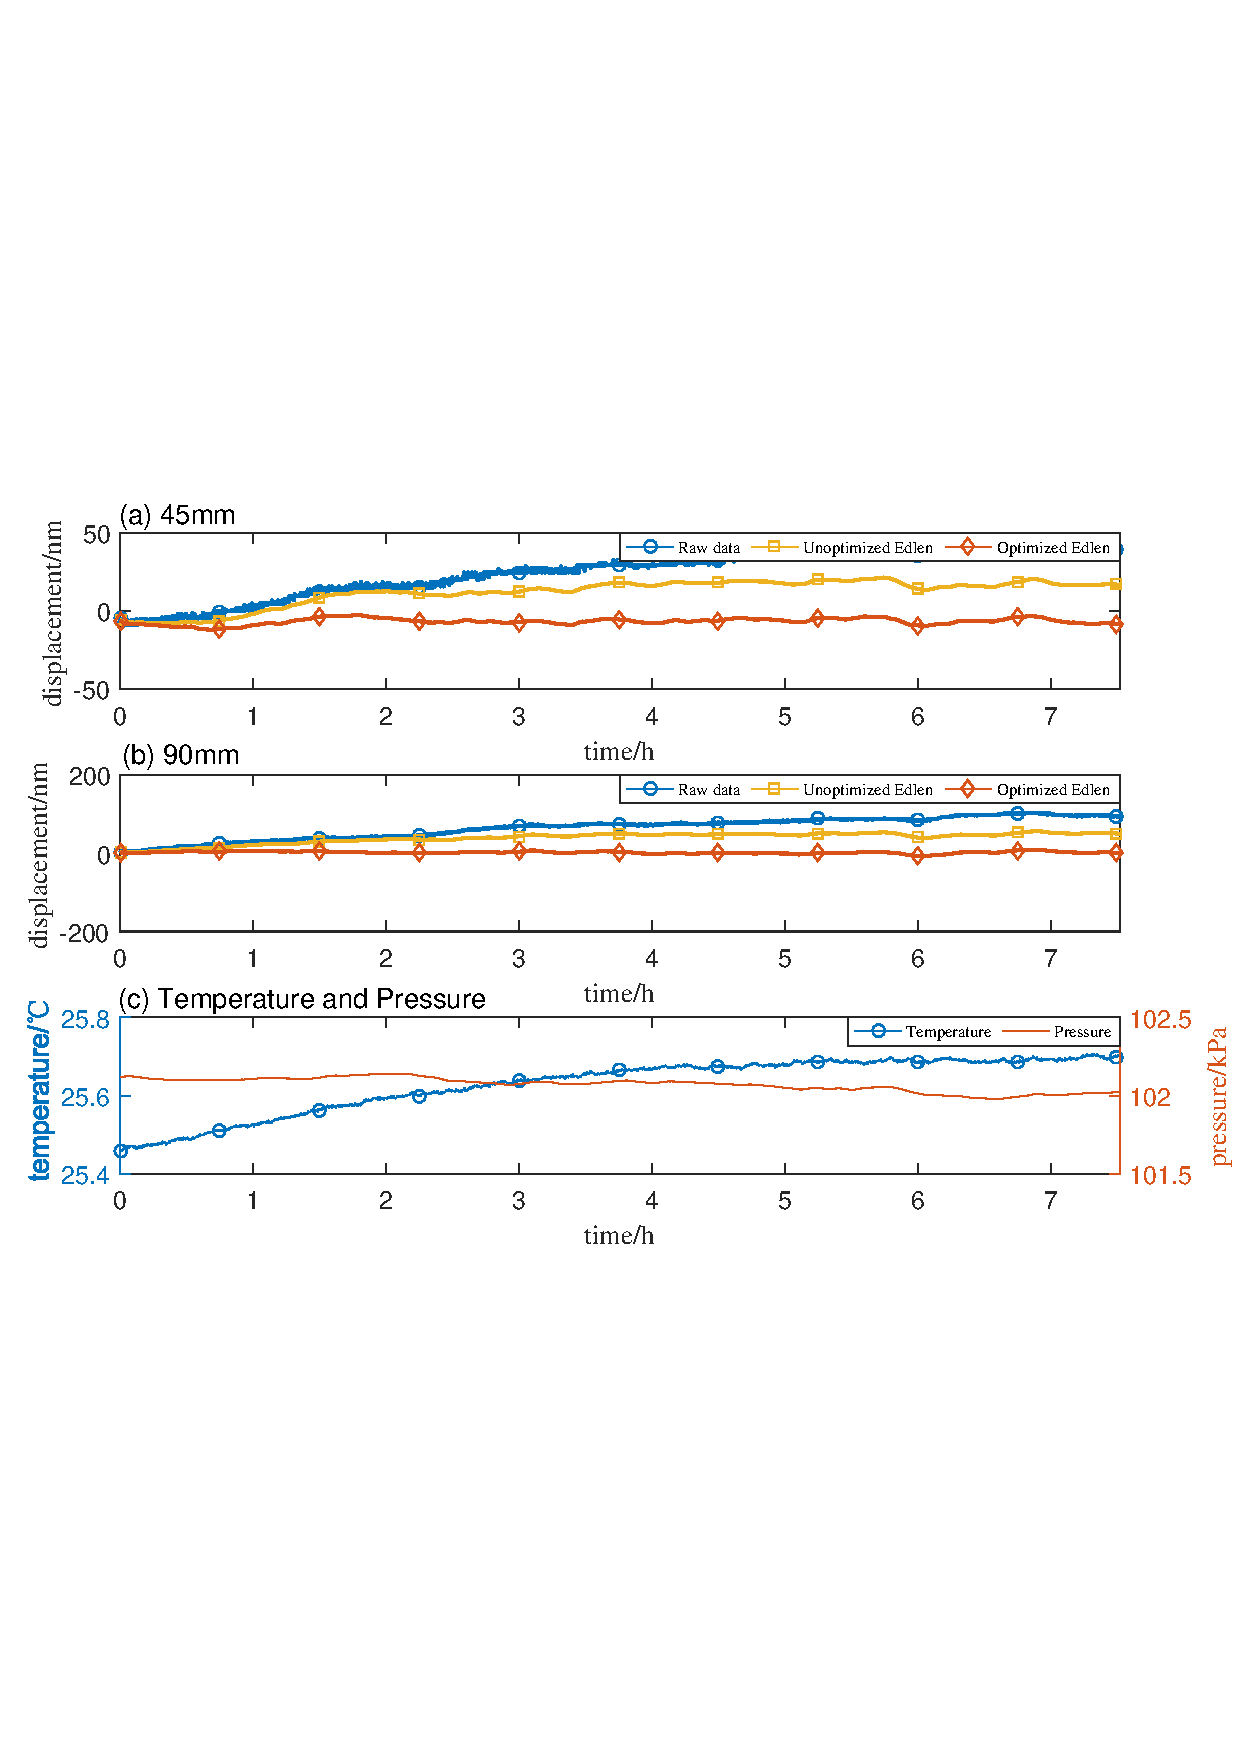
\includegraphics[width=14cm]{fig/4-fig/edpso_长时测量实验数据.pdf}
  \caption{粒子群算法优化后的长时测量补偿效果}
  \label{fig:粒子群算法优化后的长时测量补偿效果}
\end{figure}

同时,从数据中可以发现,测量臂长度为$90nm$的数据经过粒子群算法优化后的补偿残差$3.6700nm$是小于$45nm$的$6.8308nm$,可能原因有:
\begin{enumerate}
  \item 由于粒子群算法在训练过程中使用的是$90nm$的测量数据,并且该组试验的测量时间较长,使得粒子群算法较好地挖掘了数据中潜在的规律,达到比较完美的补偿效果。
  \item $45nm$的测量数据发生了过补偿。
  \item 由于环境补偿后的残差较小,所以可能由于随机误差的干扰。
\end{enumerate}

需要特别说明的是,从其他未给出的实验数据以及下文给出的大范围温度变化测量的结果分析,比较大的可能是由于随机误差的干扰。
\subsection{大范围温度变化测量}
对前文所述的大范围温度变化测量的实验数据也是用粒子群算法优化后再进行补偿,结果如图\ref{fig:粒子群算法优化后的大范围温度变化测量补偿效果}所示,虽然采样时长以及温度变化范围都增加了,但是粒子群算法的优化效果依旧显著。从数据层面分析,使用粒子群算法进行优化之后再进行补偿,测量臂长度为$45nm$的干涉仪的残留均方根误差从$153.6245nm$降低为$29.3458 nm$,而$90nm$长度的则从$176.6071nm$降低为$48.4996nm$,两者残差的差值仍有$19.1538nm$,相较于未优化前的差值$28.5849nm$有着一定提升,这说明环境误差的补偿效果得到一定改善,但是不同测量臂长度下的残差仍然不可以认为是相等的,说明该组实验数据哪怕经过整段式粒子群算法的优化,其补偿效果也只是提升了,并未像前两组实验数据那样得到精准且完全的补偿。
\begin{figure}[htb]
  \centering
  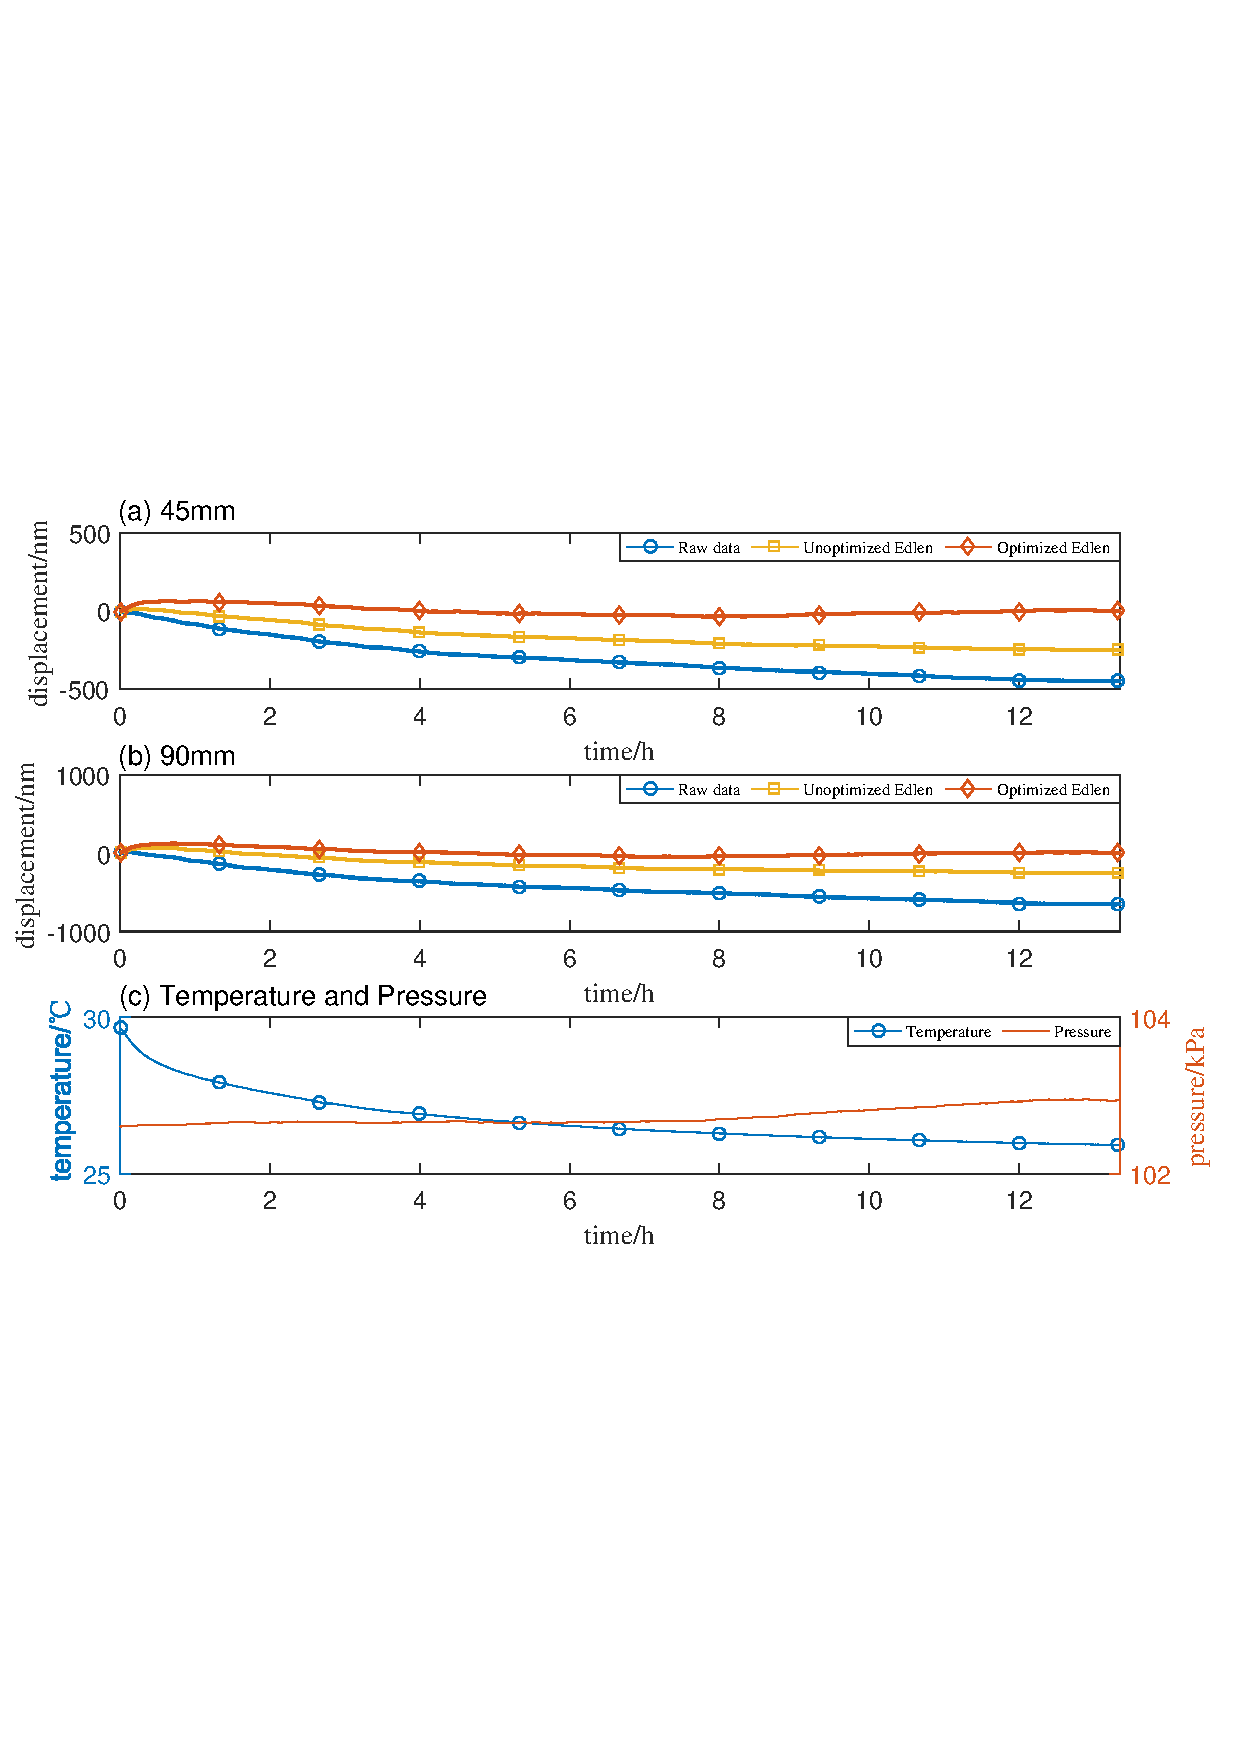
\includegraphics[width=14cm]{fig/4-fig/edpso_大范围温度变化测量数据.pdf}
  \caption{粒子群算法优化后的大范围温度变化测量补偿效果}
  \label{fig:粒子群算法优化后的大范围温度变化测量补偿效果}
\end{figure}

但是从上述的分析数据中可以看出,该组的温度变化以及测量时间均比长时测量实验中长,但是经过粒子群算法优化后再进行补偿得到的残差值,并未出现长时测量实验中:测量臂长度为$45nm$的补偿残差大于测量臂长度为$90nm$的补偿残差,这进一步验证了长时测量实验中出现该现象的原因是由于偶然的随机误差,难以复现。

前$0.8h$时间内的过补偿现象变得更严重了,经粒子群算法优化后的补偿结果的凸起高度从$70nm$增大到了约$120nm$,但是使用粒子群算法优化后在整个$12.5h$测量时间内的补偿效果是改善的,这说明粒子群算法已经比较完全地挖掘出了Edlen公式的补偿性能,只是在大温度梯度的情况下,可能引入了其他误差因素,导致线性形式的Edlen公式无法适用。

\subsection{局限性}
